% This is a basic Math Paper

\documentclass[11pt]{article}

% Preamble

\usepackage[margin=1in]{geometry}
\usepackage{amsfonts, amsmath, amssymb}
\usepackage{fancyhdr, float, graphicx}
\usepackage[utf8]{inputenc} % Required for inputting international characters
\usepackage[T1]{fontenc} % Output font encoding for international characters
\usepackage{fouriernc} % Use the New Century Schoolbook font
\usepackage[nottoc, notlot, notlof]{tocbibind}
\usepackage[hidelinks]{hyperref}

% Header and Footer
\pagestyle{fancy}
\fancyhead{}
\fancyfoot{}
\fancyhead[L]{\textit{\Large{Working of Turbines in a Thermal Power Plant}}}
%\fancyhead[R]{\textit{something}}
\fancyfoot[C]{\thepage}
\renewcommand{\footrulewidth}{1pt}

\begin{document}	
	\begin{titlepage} 
		\centering 
		
		%---------------------------NAMES-------------------------------
		
		\huge\textsc{
			MIT World Peace University
		}\\
	
		\vspace{0.75\baselineskip} % space after Uni Name
		
		\LARGE{
			Basic Mechanical Engineering\\
			First Year B. Tech, Trimester 1
		}
		
		\vfill % space after Sub Name
		
		%--------------------------TITLE-------------------------------
		
		\rule{\textwidth}{1.6pt}\vspace*{-\baselineskip}\vspace*{2pt}
		\rule{\textwidth}{0.6pt}
		\vspace{0.4\baselineskip} % Whitespace above the title
		
		
		
		\huge{\textsc{
				Working and Operation of Turbines used in a Thermal Power Plant
			}} \\
		
		
		
		\vspace{0.5\baselineskip} % Whitespace below the title
		\rule{\textwidth}{0.6pt}\vspace*{-\baselineskip}\vspace*{2.8pt}
		\rule{\textwidth}{1.6pt}
		
		\vspace{1\baselineskip} % Whitespace after the title block

		%--------------------------SUBTITLE --------------------------	
			
		\LARGE\textsc{
			Experiment 11\\Practical Report
		} % Subtitle or further description
		\vfill
		
		%--------------------------AUTHOR-------------------------------
		
		Prepared By
		\vspace{0.5\baselineskip} % Whitespace before the editors
		
		\Large{
			109050. Atharva Tanavade \\
			109051. Balraj Tavanandi \\
			109054. Krishnaraj Thadesar \\
			Division 9, Batch I3
		}
		
		
		\vspace{0.5\baselineskip} % Whitespace below the editor list
		\today

	\end{titlepage}

\tableofcontents
\thispagestyle{empty}
\clearpage
\setcounter{page}{1}

\section{Objective}
To study the difference components used in a Thermal Power Plant, learn in detail about the types and components of the relevant turbines and to understand its working and significance. 
\section{Theory}

\subsection{Thermal Power Plant}
Thermal power plant is the most conventional source of electric power generation.\\ At present about 55\% of total electricity production in India is from Coal Based Thermal Power Stations. A coal based thermal power plant converts the chemical energy of the coal into electrical energy. This is achieved by burning coal in the furnace releasing the heat of combustion, which raises steam in the boiler, the high pressure high temperature steam is expanded through the turbine rotating it which is coupled to a generators converting mechanical energy into electrical energy.\\

\subsection{Working of a Thermal Power Plant}

The working fluid in the thermal power plant is water or steam. The ideal thermodynamic cycle for the thermal power plant is \textbf{Rankine Cycle.} \\

Referring to Figure. \ref{tpp}, the process \textit{$ 1-2 $} is pumping water from condenser pressure to boiler pressure. In boiler the water is heated at constant pressure first to saturation temperature \textit{(process 2-3)}, then it is converted into steam \textit{(phase transformation process 3- 4)} and then it is superheated (\textit{process 4-5}). The superheated steam then expands in turbine from boiler pressure to condenser pressure (\textit{process 5-6}) producing mechanical work. The saturated or unsaturated steam coming from turbine condenses in the condenser (\textit{process 6-1}). The turbine is coupled with generator converting the mechanical energy into electrical energy. \\


\begin{figure}[H]
	\centering
	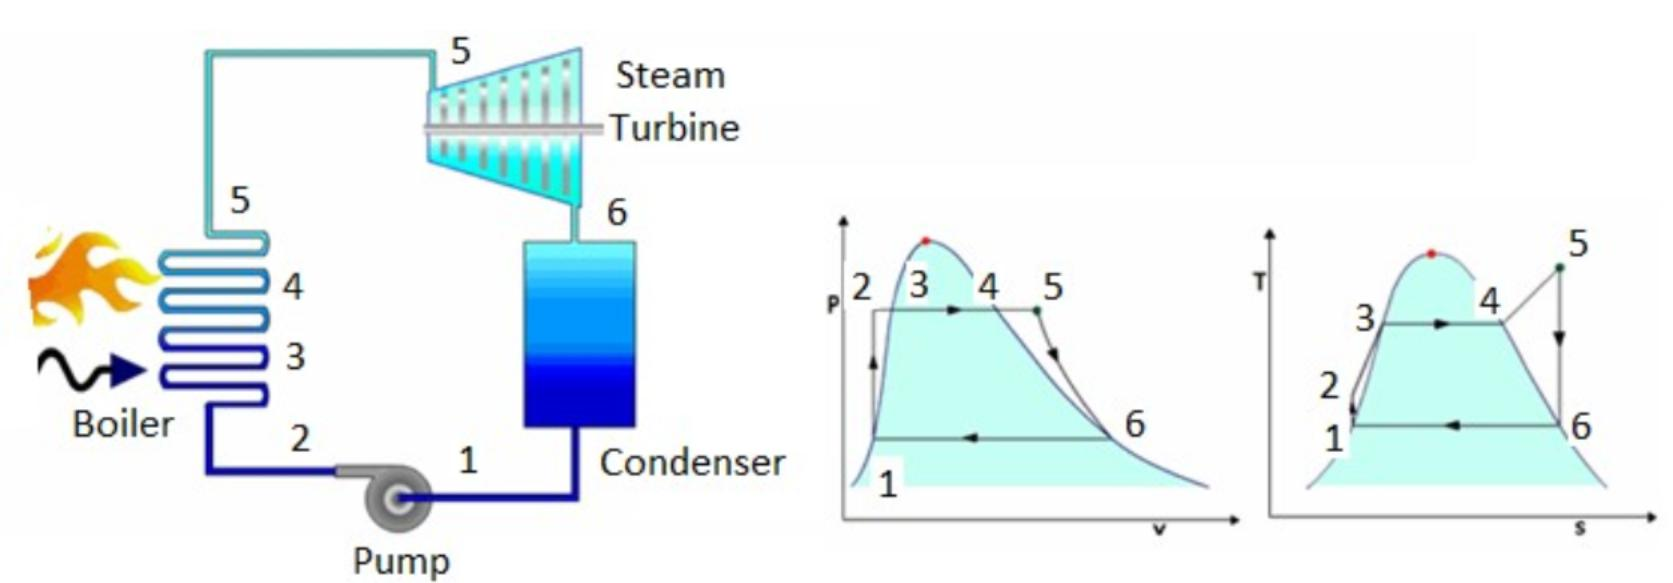
\includegraphics[scale=0.28]{Thermal Power Plant.jpg}
	\caption{Working of a Thermal Power Plant}
	\label{tpp}
\end{figure}


In two stages compressor air is partially compressed in low-pressure cylinder this air is
passed through between the first stage and the second stage so that air at the inlet of the second stage is at lower temperature than the first stage outlet. This is done to reduce the work of compressor in second stage. Final compression is completed in the second stage. Also the compressors are provided with clearance volume, two stage compressors can achieve higher volumetric efficiency than a single stage compressor because of lower compression per stage. As the compressed air is used in a wide range in industrial, domestic, aeronautics Fields, etc. so compressors are applied in a wide range. Compressors are used where the air is required at high pressure.\\


Important components of Thermal Power Plant:

\begin{enumerate}
	\item Boiler
	\item Steam Turbine
	\item Condenser
	\item Pump
\end{enumerate}

\subsection{Boiler}
A Boiler or steam generator essentially is a container into which water can
be fed and steam can be taken out at desired pressure, temperature and flow. This calls for
application of heat on the container. For that the boiler should have a facility to burn a fuel and release the heat. The functions of a boiler thus can be stated as:-

\begin{enumerate}
	\item To convert chemical energy of the fuel into heat energy. 
	\item To transfer this heat energy to water for evaporation and to steam for superheating. 
\end{enumerate}

The Basic Components of a Boiler are:
\begin{enumerate}
	\item Furnace and Burners
	\item Steam and Superheating.
\end{enumerate}

\subsection{Turbines}
Steam turbines have been used predominantly as prime mover in all
thermal power stations.\\


\begin{figure}[H]
	\centering
	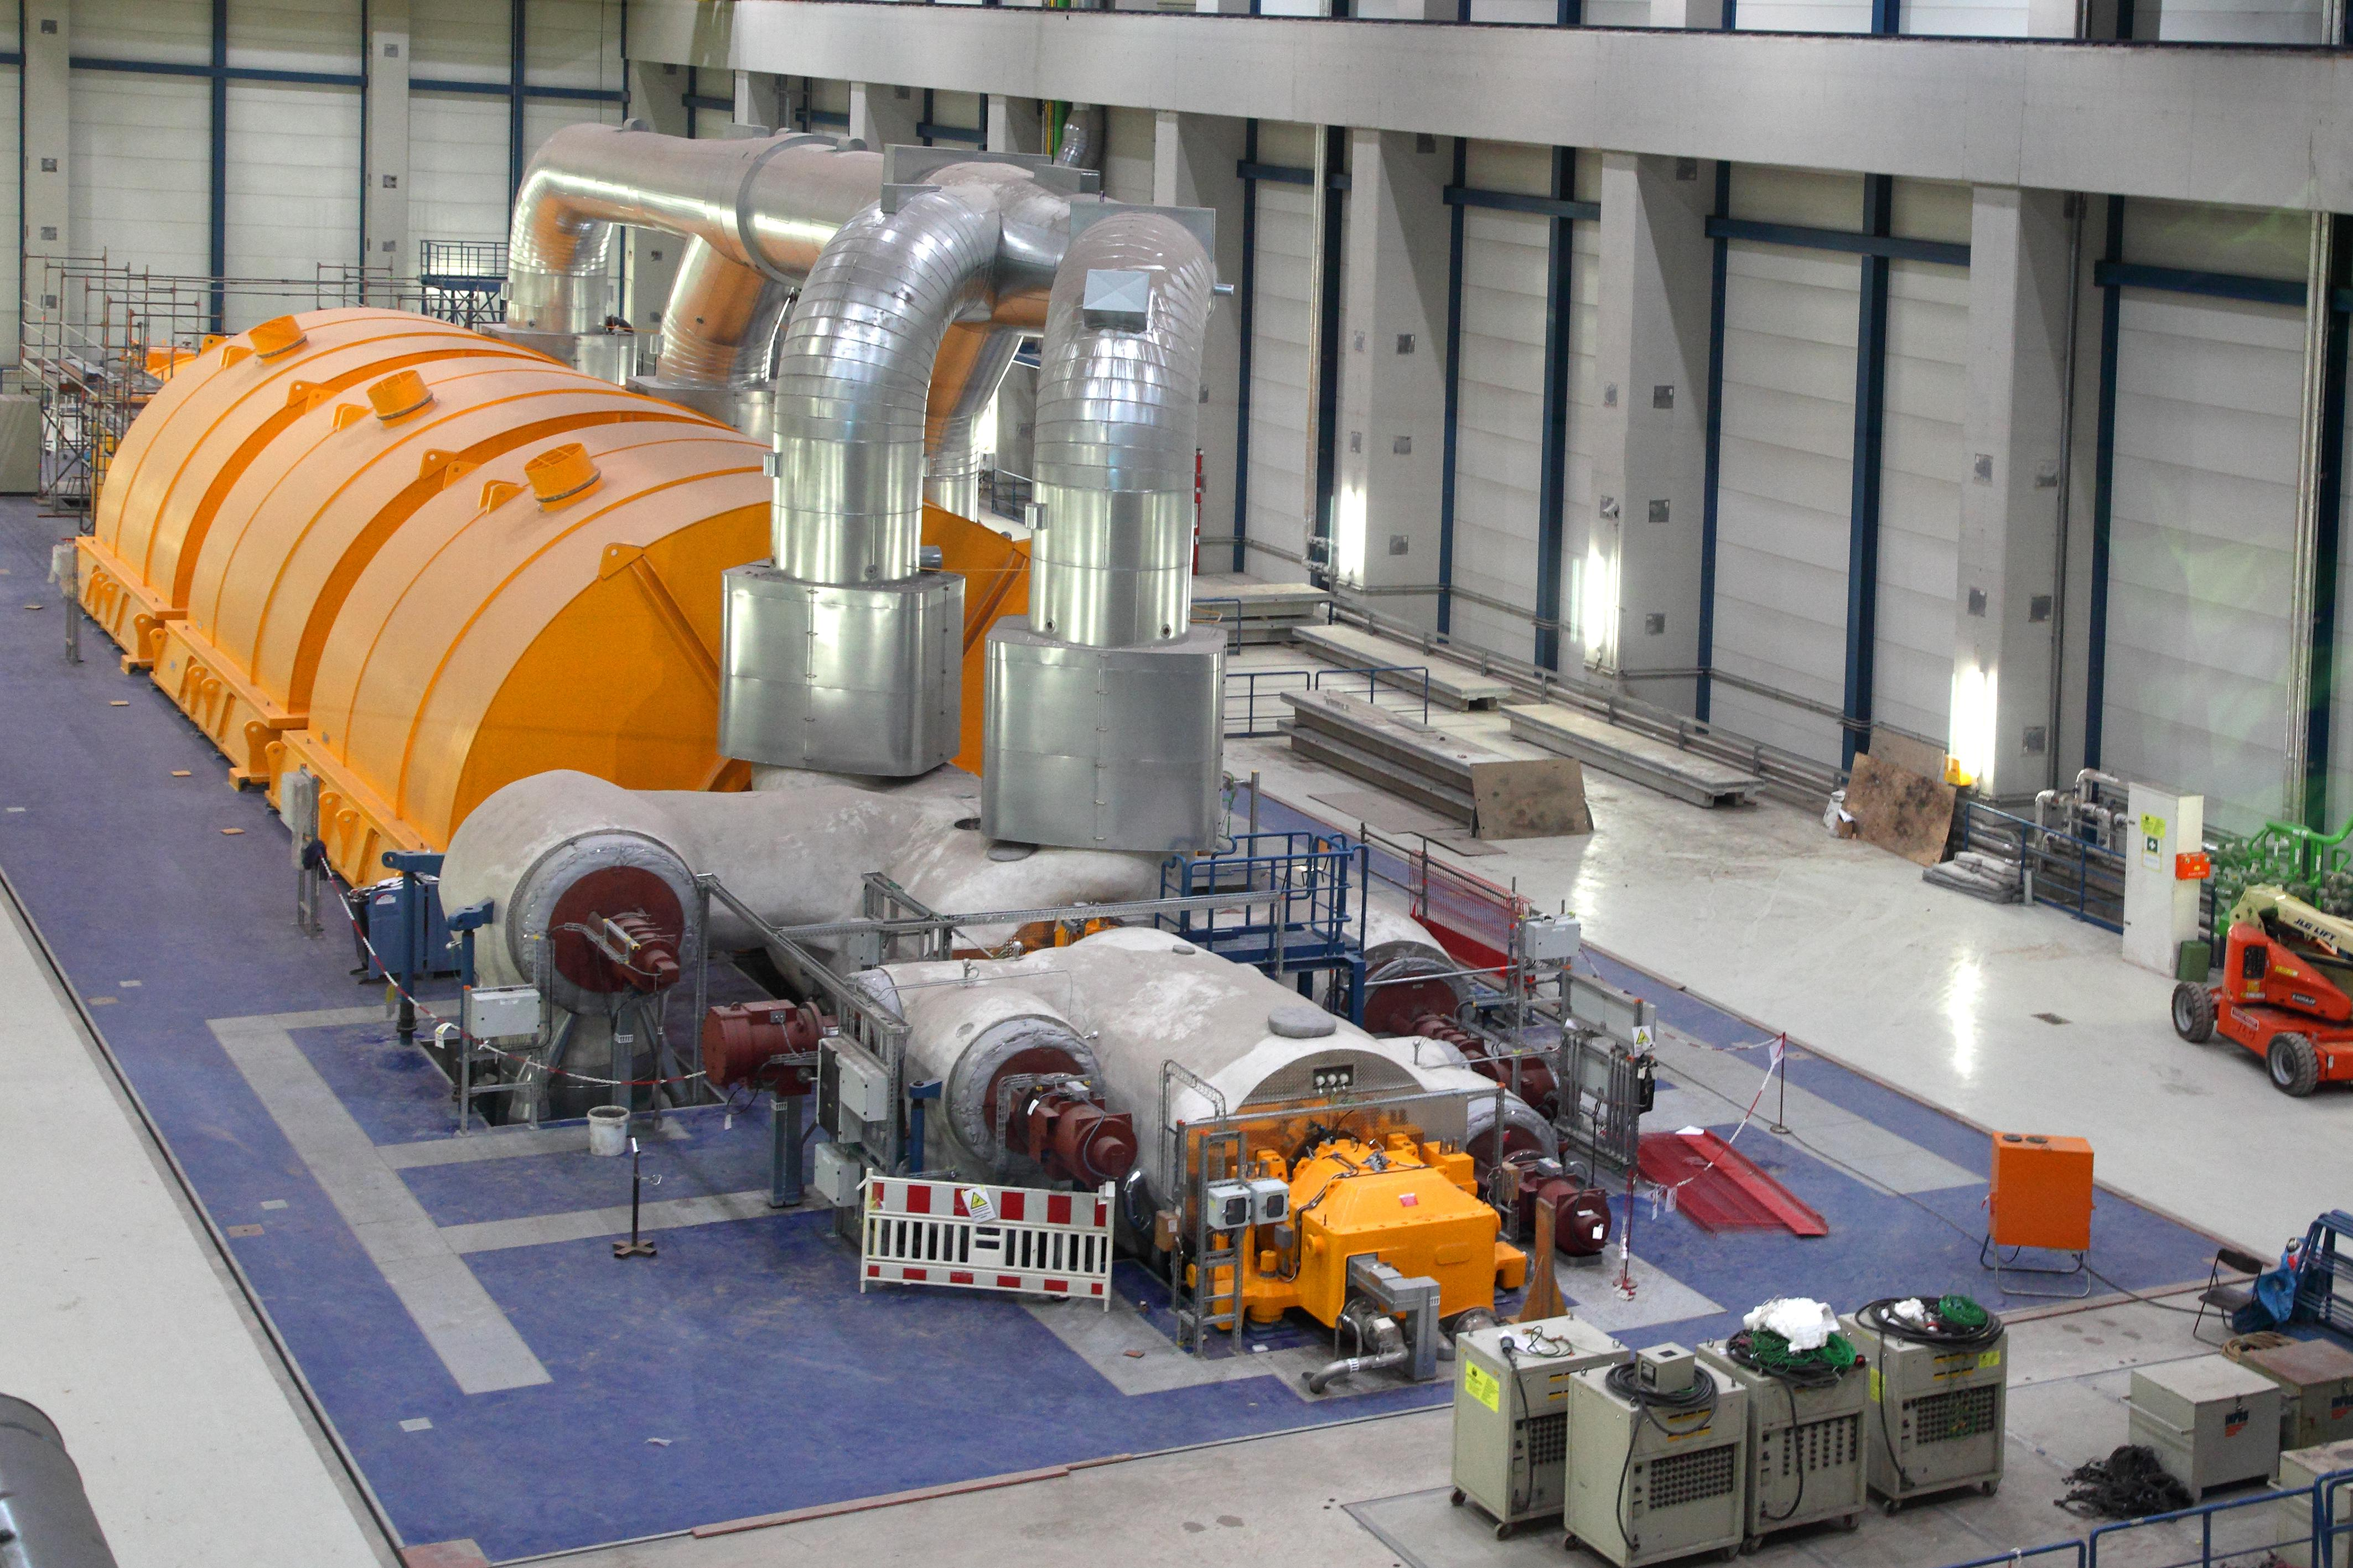
\includegraphics[scale=0.06]{turbine.jpg}
	\caption{An Thermal Power Plant Turbine}
	\label{turbine}
\end{figure}

The steam turbines are mainly divided into two groups: -
\begin{enumerate}
	\item Impulse Turbine
	\item Impulse-Reaction Turbine
\end{enumerate}

\textit{Turbines and their types will be discussed in detail further in the Experiment. 
}

\subsection{Condenser}
The condenser condenses the steam from the exhaust of the turbine into liquid to
allow it to be pumped. If the condenser can be made cooler, the pressure of the exhaust steam
is reduced and efficiency of the cycle increases. The functions of a condenser are:-


\begin{enumerate}
	\item To provide lowest economic heat rejection temperature for steam
	\item To convert exhaust steam to water for reserve thus saving on feed water requirement.
	\item To introduce make up water.
\end{enumerate}


\section{Turbines and Their types}

Considering how the fluid flow acts on the turbine blades causes Turbines to be classified into two categories: impulse and reaction, which are then further classified into different types based on their use in Hydro or Thermal Power plants. 

\subsection{Impulse Turbine used in a Hydro Power plant}
\begin{figure}[H]
	\centering
	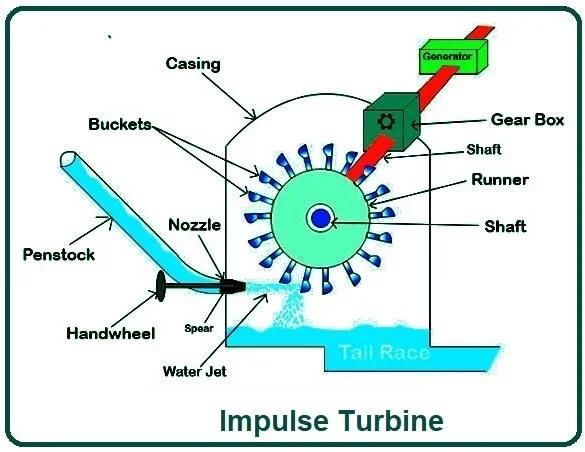
\includegraphics[scale=0.6]{impulse turbine.jpg}
	\caption{An Impulse Turbine}
	\label{it}
\end{figure}

\textit{Impulse turbines are defined as turbines in which high-velocity jets of water or steam collide with the blades of the turbine to rotates the turbine and produce electricity using this winding. The impulse turbine is so named because it acts on the impulse force created for the striking blade of the water jet.}\\


In impulse turbines, water hits the blade tangentially; hence it is also known as a tangent flow turbine. Impulse turbines are suited for high head and low discharge of water. This means that it is used when the amount of water flow is small, and there is high pressure due to the high location of the water head.\\

The impulse turbine changes the velocities of a water jet. The jet is mounted on the winding blade of the turbine, which changes the direction of flow. A change in impulse (impulse) causes a force on the turbine blade. As the turbine is spinning, the force acts through a distance (work), and the oblique water flow is released with less energy.  \\



\subsubsection{Components of on Impulse Turbine:}

\begin{enumerate}
	\item Penstock: The penstock impulse is a channel or pipe to deliver water to the turbine. Using this penstock, water is brought to the turbine at the high head. This penstock is associated with water reserves. The water reservoir is typically several meters high.
	\item Nozzle: The nozzles are used to increase the kinetic energy of the water and to spray water to the blades of the turbine. This nozzle forms a jet with high velocity. This indicates the flow of water towards the blade in a particular direction. In an impulse turbine, single or multiple nozzles may be used.
	\item Runners: The runner is a circular disk mounted on a rotating shaft. This rotating shaft is known as a rotor. On the runner, there are also cup-shaped blades that are evenly rounded. The cup-shaped blade, also known as a bucket, is mounted on the runner. These buckets are placed in such a way that these buckets are spread evenly.
	\item Bucket: Buckets are cup or spoon-shaped blades of a turbine. The bucket is placed around the circumference of the runner so that the pressurized fluid collides with the bucket; the bucket will gain momentum from the fluid and helps the runner rotate using fluid motion.
	\item Casing: In an impulse turbine, the casing is used to prevent water splatter and to direct the spillway so that water does not dissipate. This cover is also used to protect components from the external environment. The cover is usually made of cast iron.
	\item Braking Jet: The braking jets are used to stop the turbine blades after the water supply is shut off from the nozzle. Turbine blades continue to rotate even after the water supply from the nozzle is shut down due to inertia. Therefore, the blade is struck from the opposite side of the turbine blade to prevent the blade from rotating immediately.
\end{enumerate}

\subsubsection{Working Principle of Impulse Turbine:}


\begin{figure}[H]
	\centering
	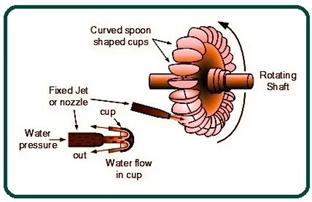
\includegraphics[scale=1]{impulse turbine 2.jpg}
	\caption{Working of the nozzle of the Impulse Turbine}
	\label{it2}
\end{figure}


In this turbine, the static pressure inside the runners is constant, and the turbine runner is at atmospheric pressure. The runner rotates in the air, and the blade is sprayed through the nozzle to exchange energy with the turbine. Jet nozzles or a series of nozzles direct high-speed flow to the blades, which are usually in the shape of a bucket or cup. Therefore, only the pressure changes in the nozzle.\\ 

The application of curved blades is to change the velocity of flow. This strike causes a change in speed, and a force is applied to the turbine blades based on the law of energy interaction. According to Newton’s second law of motion, forces obtained through a motion of the fluid depends on two factors: \textit{the mass of the fluid entering the turbine and the change in the velocity of the fluid between the turbine inlet and outlet}. As there is no change in the fluid mass, only the change in velocity is taken into account in the calculation of the force applied to the runner.\\

Thus, in the power generation process in impulse turbines, the following steps are applied.
 
\begin{enumerate}
	\item The stored water flows upstream from a source through the penstock to reach the nozzle.
	\item The potential energy of water inside the nozzle is converted into kinetic energy and injected into the blade or bucket; Thus, the runner rotates.
	\item The runner has a mechanism to control the flow of injected water. The spear usually plays an important role in this process.
	\item The generator connected to the shaft converts mechanical energy into electrical energy.
\end{enumerate}


\begin{figure}[H]
	\centering
	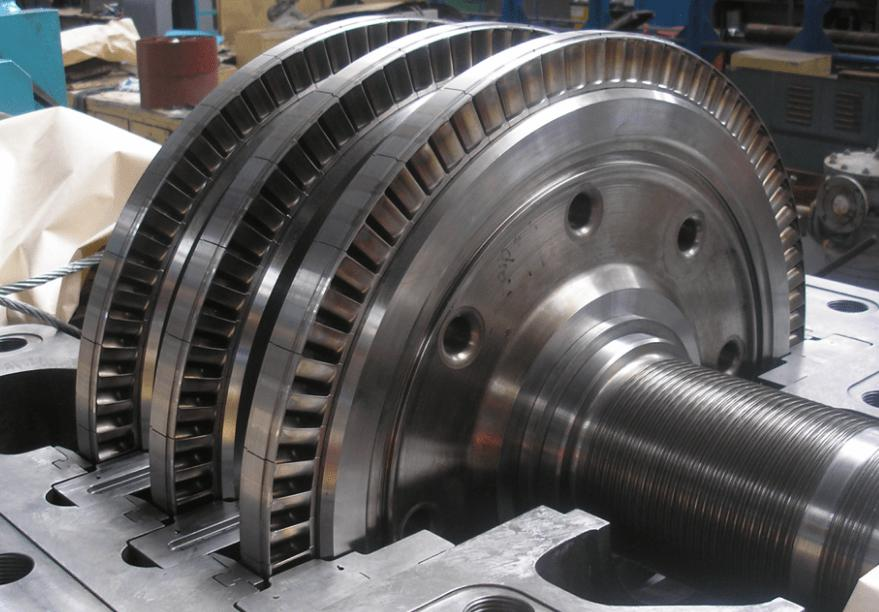
\includegraphics[scale=0.4]{impulse turbine thermal.jpg}
	\caption{An Impulse Turbine used in a Thermal Power plant}
	\label{it}
\end{figure}

\begin{figure}[H]
	\centering
	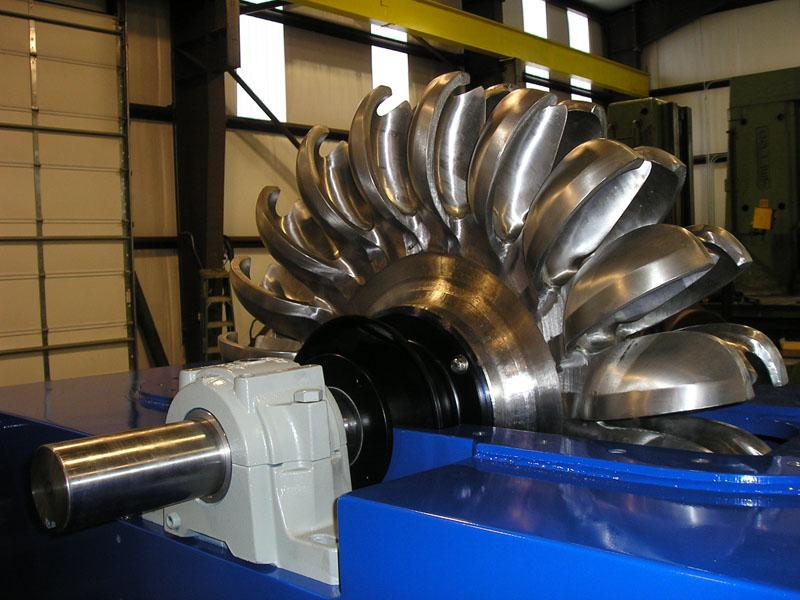
\includegraphics[scale=0.5]{impulse turbine hydro.jpg}
	\caption{An Impulse turbine used in a Hydro Power plant}
	\label{it}
\end{figure}

Impulse turbine has the ability to take all kinetic energy from water for high efficiency. After reaching the runner, water is discharged into the atmosphere from the bottom of the turbine housing; therefore, there is no suction at the bottom of the turbine. Here you can see schematically how an impulse turbine works in the process of extracting the kinetic energy of water as well as the power from its components.

\subsection{Reaction Turbines}

Reaction turbines are a type of turbine that develops torque by reacting to the gas or fluid’s pressure or mass. The operation of reaction turbines is described by Newton’s third law of motion (action and reaction are equal and opposite).

In a reaction turbine, the water enters the wheel under pressure and flows over the vanes, As the water, flowing over the vanes, is under pressure, therefore wheel of the turbine runs full and may be submerged below the tailrace or may discharge into the atmosphere.\\

\begin{figure}[H]
	\centering
	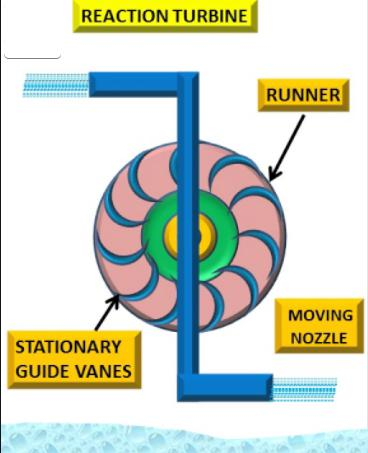
\includegraphics[scale=0.8]{reaction turbine.jpg}
	\caption{A Reaction Turbine}
	\label{it}
\end{figure}


\subsubsection{Parts of Reaction Turbine}

\begin{enumerate}
	\item Spiral casing: The water, from a pipeline, is distributed around the guides ring in a casing. This casing is designed in such a way that its cross-sectional area goes on reducing uniformly around the circumference. 
	The cross-sectional area is maximum at the entrance and the minimum at the tip. As a result of this, the casing will be of the spiral casing or scroll casing.
	\item Guide mechanism: The guide vanes are fixed between two rings in the form of a wheel. This wheel is fixed in the spiral casing. The guide vanes are properly designed in order to:
		\begin{enumerate}
			\item To allow the water to enter the runner without shock.
			\item Allow the water to flow over them, without forming eddies.
			\item Allow the required quantity of water to enter the turbine. (this is done by adjusting the opening of the vanes).
		\end{enumerate}

	All the guide vanes can rotate about their respective pivots, which are connected to the regulating ring by some mechanical means. The regulating ring is connected to the regulating shaft by means of two regulating rods.\\	
	The guide vanes may be closed or opened by rotating the regulating shaft, Thus allowing the required quantity of water to flow according to the need. The regulating shaft is operated by means of a governor, whose function is to govern the turbine (i.e., to keep the speed constant at varying loads). The guide vanes are generally made of cast steel.
	\item Turbine runner: The runner of a reaction turbine consists of runner blades fixed either to a shaft or rings, depending upon the type of turbine. The blades are properly designed, in order to allow the water to enter and leave the runner without	shock.\\
	The runner is keyed to a shaft, which may be vertical or horizontal. If the shaft
	is vertical, it is called a vertical turbine. Similarly, if the shaft is horizontal, it is called a horizontal turbine\\
	The surface of the runner is made very smooth. The runner may be cast in one piece it may be made of separate steel plates and welded together. For low heads, the runner may be cast iron. But for high heads, the runner is made of steel or alloys. when the water is chemically impure, the runner is made of special alloy.
	
	\item Draft tube: The water, after passing through the runner, flows down through a tube called draft tube. it is, generally, drowned approximately 1 m below the tailrace level. A draft tube has the following functions: 
\end{enumerate}


\subsubsection{Types of Reaction Turbine}

The reaction turbines may be classified into the following three types, depending upon the direction of flow of water through the wheel. 

Types of Reaction Turbine are:
\begin{enumerate}
	\item Radial flow turbines: In such turbines, the flow of water is radial (i.e., along with the radius of the wheel). The radial flow turbines may be further sub-division into the following two classes:
		\begin{enumerate}
			\item Inward Flow Turbines:
				\begin{enumerate}
					\item In such turbines, the water enters the wheel at the outer periphery and then flows inwards(i.e. towards the centre of the wheel).
					\item Here the runner is surrounded by a guide mechanism.
					\item In this turbine, the outer diameter of the runner is the inlet and the inner diameter is the outlet.
				\end{enumerate}
			\item Outward Flow Turbines
				\begin{enumerate}
					\item In such turbines, the water enters at the centre of the wheel and then flows outwards (i.e., towards the outer periphery of the wheel).
					\item Here guide mechanism is surrounded by the runner.
					\item In this turbine, the inner diameter of the runner is the inlet and outer diameter is an outlet.
				\end{enumerate}
		\end{enumerate}
	\item Axial flow turbines: In such turbines, the water flows parallel to the axial of the wheel. Such turbines are also called parallel flow turbines. They can be of the \textit{Kaplan or Propeller Turbine type.}
	
	\item Mixed flow turbines: The Francis turbine is a type of water turbine that was developed by James B. Francis. It is an inward flow reaction turbine that combines radial and axial flow concepts.\\
	They operate in a head range of ten meters to several hundred meters and are primarily used for electrical power production and their output varies from a few kilowatts to 1000 megawatt. In this turbine the working fluid changes pressure as it moves through the turbine, giving up its energy. This types of turbines are located in between the high-pressure water source and the low-pressure water exit.
	
\end{enumerate}


\begin{figure}[H]
	\centering
	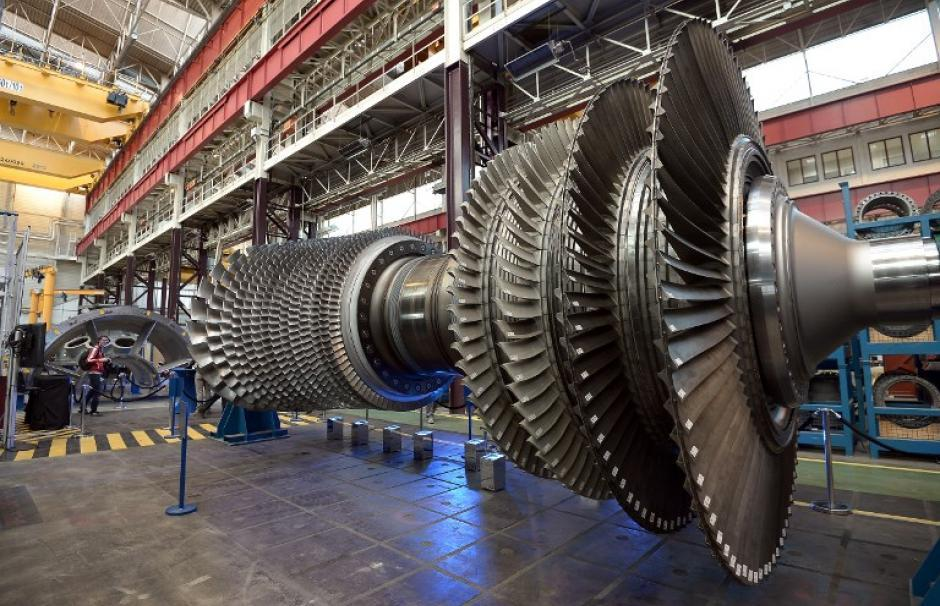
\includegraphics[scale=0.4]{reaction turbine thermal.jpg}
	\caption{A Reaction Turbine used in a Thermal Power plant}
	\label{it}
\end{figure}

\begin{figure}[H]
	\centering
	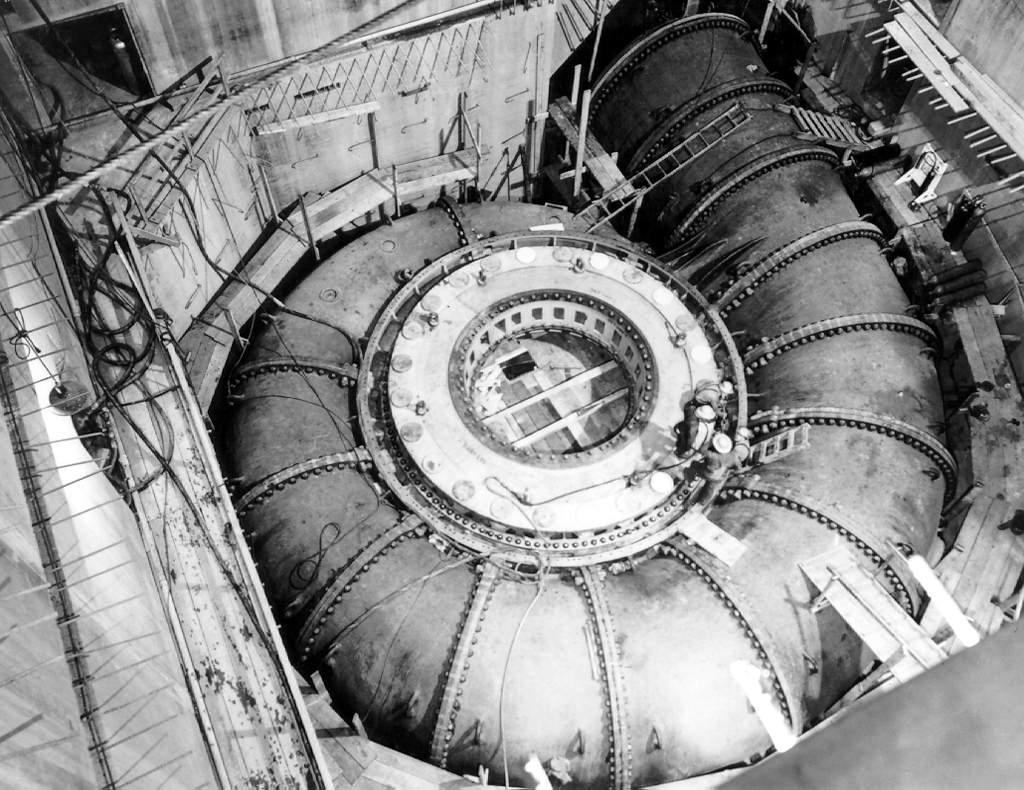
\includegraphics[scale=0.4]{reaction turbine hydro.jpg}
	\caption{A Francis Reaction Turbine used in a hydro Power plant}
	\label{it}
\end{figure}

\section{The Difference between a Reaction and an Impulse Turbine}


\begin{enumerate}
	\item In impulse turbine the steam flows through the nozzle and strikes on the moving blades. In reaction turbine steam first flows through the guide mechanism and then flows through the moving blades.
	\item In impulses turbine, steam strikes on the moving blades with kinetic energy only. But in the reaction turbine, the steam which glides over the moving blades possesses both pressure and kinetic energy.
	\item In impulse turbine the pressure of steam remains constant during its flow through the moving blades. But in reaction turbine, the pressure of steam reduces during its flow through the moving blades.
	\item In impulse turbine the steam may or may not be admitted to the whole circumference. In reaction turbine the steam must be admitted to the whole circumference.
	\item The blades of the impulse turbine are symmetrical where as in reaction turbine it is not symmetrical.
	\item The relative velocity of steam in impulse turbine remains constant but in Reaction turbine it increases while gliding over the blades.
	\item For the same power developed, the number of stages required in impulse turbine is less where as in reaction turbine the number of stages required is more.
	\item The steam flow in impulse turbine is radial to the turbine wheel where as in reaction turbine steam flow is radial and axial to the turbine wheel.
	\item If we talk about the maintenance work, then impulse turbine has less maintenance work as compared with the reaction turbine.
	\item Impulse turbine is suitable where discharge is low and reaction turbine is suitable for medium and high discharge.
	\item Pelton wheel is the example of impulse turbine whereas Francis turbine, Kaplan turbine etc. are the examples of reaction turbine
\end{enumerate}

\begin{figure}[H]
	\centering
	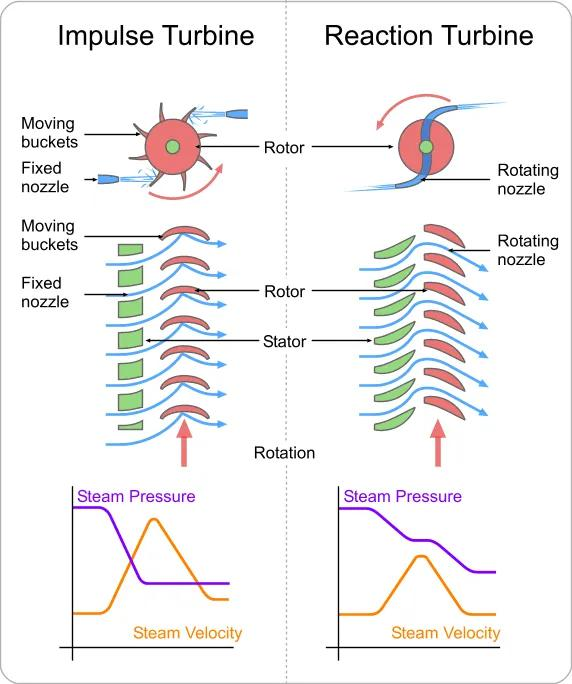
\includegraphics[scale=0.6]{difference.jpg}
	\caption{A Reaction Turbine}
	\label{it}
\end{figure}




\section{Conclusion}
The Various components of a Thermal Power Plant were studied and understood. Turbines and their types were discussed, and their working and significance was understood in detail. 
\end{document}









